\chapter{\leavevmode \newline Results}
\label{chap:Results}

This chapter presents simulation-based validation of \algoname, designed to assess its performance in a variety of terrain scenarios. The experiments evaluate \algoname\ in a variety of terrain scenarios that simulate challenges encountered during planetary exploration. These scenarios are designed to demonstrate the algorithm’s core capabilities: its ability to expand safe regions under uncertainty, navigate around high-risk areas, reuse learned terrain knowledge, and perform exploratory mapping without preassigned goals. 

\section{Evaluating the Navigation Framework}

\subsection{Validation Objectives and Contribution Scope}

\algoname\ fills a gap not currently addressed by existing navigation algorithms: it enables \textbf{proprioceptive, confidence-aware, reactive navigation} in unknown, unstructured, and deformable environments where visual sensing is unreliable or unavailable.

While prior work has addressed uncertainty in terrain modeling, safe exploration, or reactive control in isolation, this framework integrates all three in a practical, simulation-validated approach. Specifically, the method combines:
\begin{itemize}
    \item Uncertainty-guided subgoal selection based on terrain risk predictions;
    \item Active expansion of a certified safe set;
    \item Real-time navigation using diffeomorphic control in non-visual, proprioceptive settings.
\end{itemize}

This section presents simulation experiments designed to demonstrate these capabilities and compare their effectiveness to relevant prior work. The most closely related work is that of \textcite{leininger2024gaussianprocessbasedtraversabilityanalysis}, which combines Sparse Gaussian Processes with RRT*-based planning, with which the differences with \algoname\ are discussed in \autoref{sec:comparison_prior}

\subsection{Simulated Planetary Terrain and Initialization}

To execute \algoname, it is assumed that a set of initial known safe points is available to form the starting safe zone. In a real-world application, the robot would be physically placed within a verified safe region and would take several initial steps around this area to collect proprioceptive data, thereby building the initial terrain model. For simulation purposes, the robot is initialized in a designated safe region, and a set of randomly sampled points from a known safe region is used to initialize the Gaussian Process model, emulating initial contact-based measurements.

The test environments are represented as two-dimensional grids, where each cell contains a value corresponding to terrain properties such as risk or traversability. For simplicity, the ground truth environment is discretized in simulation, as defining a discrete grid is considerably more straightforward than specifying a continuous ground truth function. In practical real-world applications, the underlying terrain properties are continuous; however, they are discretized for computational purposes during processing and analysis.

For ease of implementation in simulation, the parameter set is defined as the collection of all possible coordinate points within the discrete ground truth map. This representation assumes that the discrete map provides the maximum available resolution of environmental information.

Because the traversability function \( f(x) \) is only defined abstractly in the methods section, a specific interpretation must be assigned when instantiating it for simulation. In these experiments, \( f(x) \) is constructed as a scalar field encoding relative terrain strength according to an internal definition. As a result, the safety threshold \( h \) used to distinguish between safe and unsafe regions must also be selected empirically. Its role is not to enforce an externally calibrated notion of safety, but rather to define relative risk boundaries under a particular terrain encoding. Thresholds such as \( h = 1000 \) are chosen for demonstration purposes and vary across scenarios to test different aspects of algorithm behavior.

With this simulation environment in place, the following scenarios were designed to evaluate distinct capabilities of \algoname. Each experiment highlights a different navigation objective or environmental challenge relevant to planetary exploration.



\subsection{Simulation Results}

\begin{figure}[h]
    \centering
    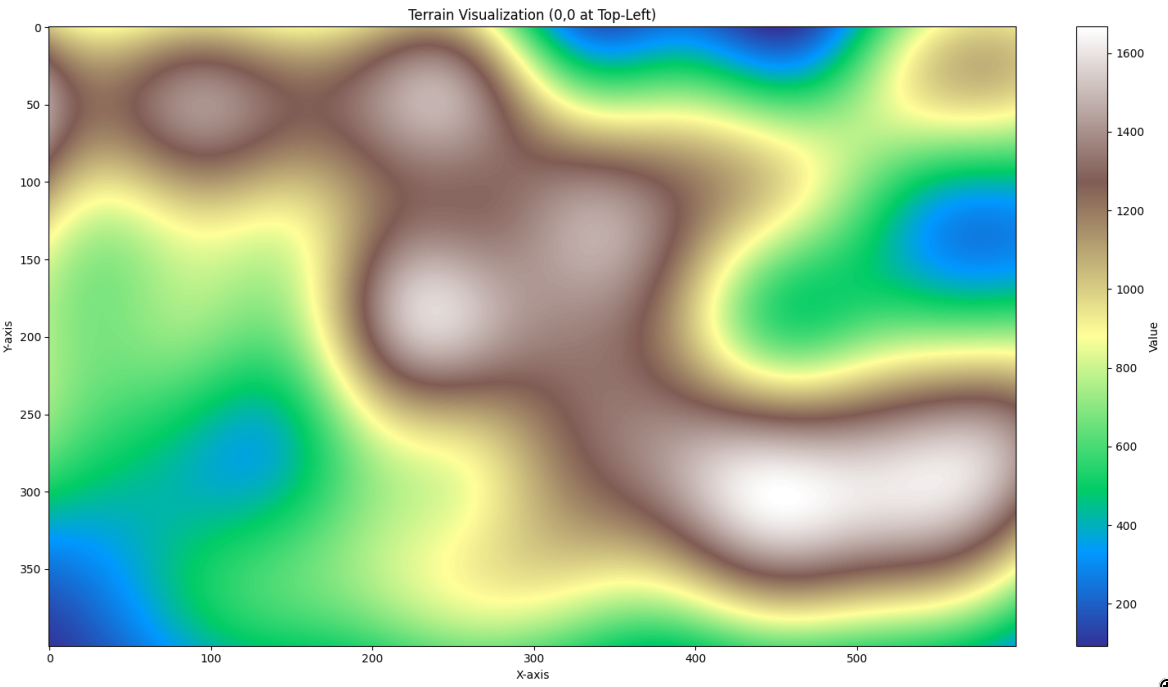
\includegraphics[width=0.7\linewidth]{figures/terrain.png}
    \caption{Visualization of ground truth risk values used in the following experiments, starting at \((230, 220)\), with a goal at \((104,82)\).}
    \label{fig:terrain}
\end{figure}

\subsubsection{Visualization Legend}

To aid in interpreting the following figures, we define the color scheme used to represent key regions and elements within the navigation environment:

\begin{itemize}
    \item \textbf{White:} Ground truth safe terrain (\( f(x) \geq h \))
    \item \textbf{Gray:} Ground truth unsafe terrain (\( f(x) < h \))
    \item \textbf{Black:} Pseudo-physical obstacles (\( \mathcal{O}_t \))
    \item \textbf{Green:} Local freespace (\( \mathcal{LF}(\mathbf{x}) \) eroded by robot radius)
    \item \textbf{Light Blue:} Safe set (\( S_t \))
    \item \textbf{Red:} Expanders (\( G_t \subseteq S_t \))
    \item \textbf{Pink:} Intermediate goal (selected \( x_t \in G_t \))
    \item \textbf{Dark Blue:} Final goal (\( x_g \))
\end{itemize}

This legend applies uniformly across all following figures in this chapter unless otherwise noted. 

\subsubsection{General Navigation}

This scenario shows the robot navigating in a scenario where the straight line path to the goal does not contain any risk zones. The robot quickly expands the safe zone as shown in \autoref{fig:easy-nav}, reaching the point in 54 iterations.

\begin{figure}[h]
    \centering
    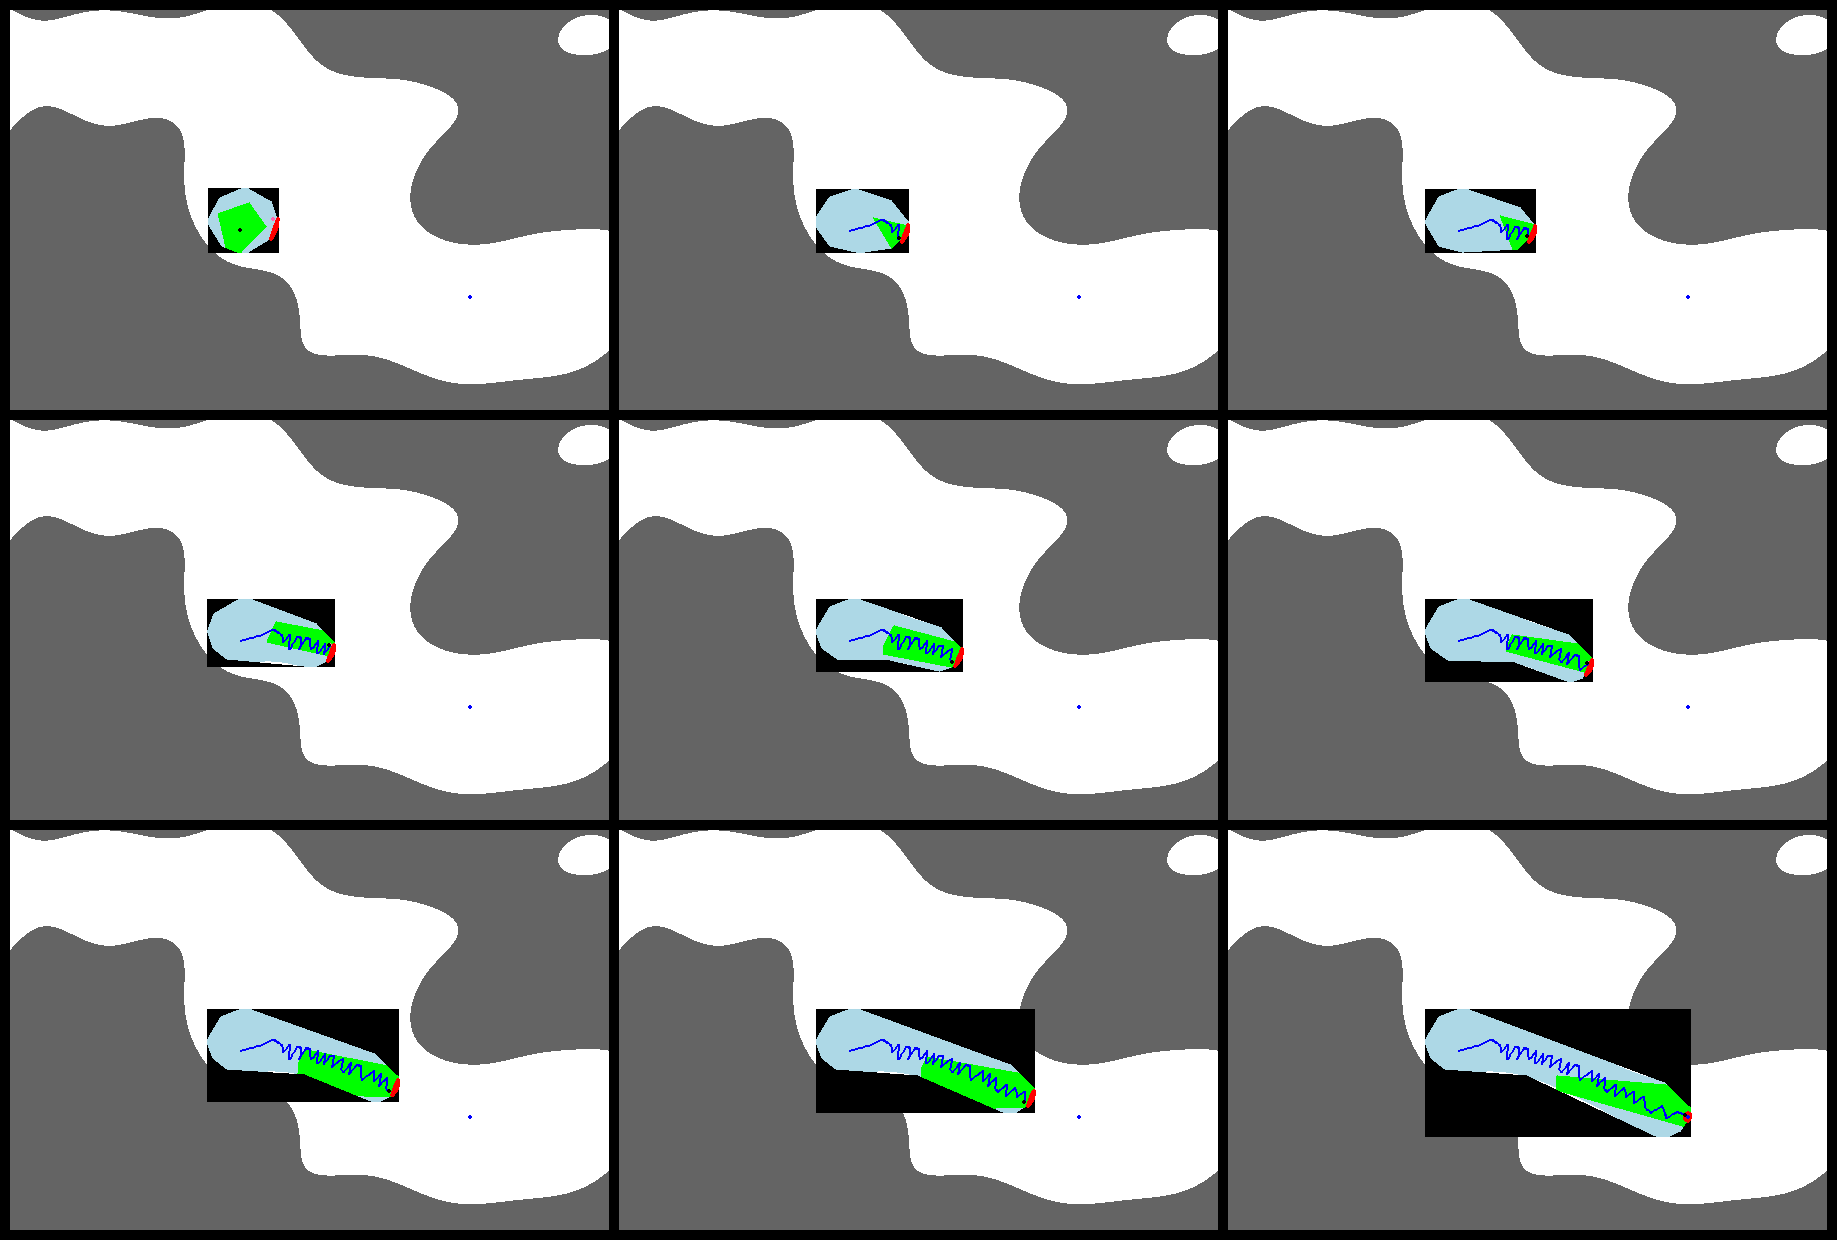
\includegraphics[width=1\linewidth]{figures/easynavigation.png}
    \caption{Nine frames showing the progression of the simple navigation task at evenly spaced intervals. Gray zones represent areas where traversability f(x) is less than 1000.}
    \label{fig:easy-nav}
\end{figure}

\subsubsection{Navigation Around a Risk Zone}
In these scenarios, the robot must reach a designated goal point located beyond a high-risk region. While the direct path to the goal intersects with terrain classified as unsafe according to the risk estimation model, the robot successfully navigates around this obstacle.

Starting with a limited known safe region, the robot employs \algoname\ to iteratively expand its accessible area until reaching the goal point. \autoref{fig:navigation} and \autoref{fig:navigation2} illustrate this process through 9 frames captured at equal intervals throughout two navigation tasks.

\begin{figure}[h]
    \centering
    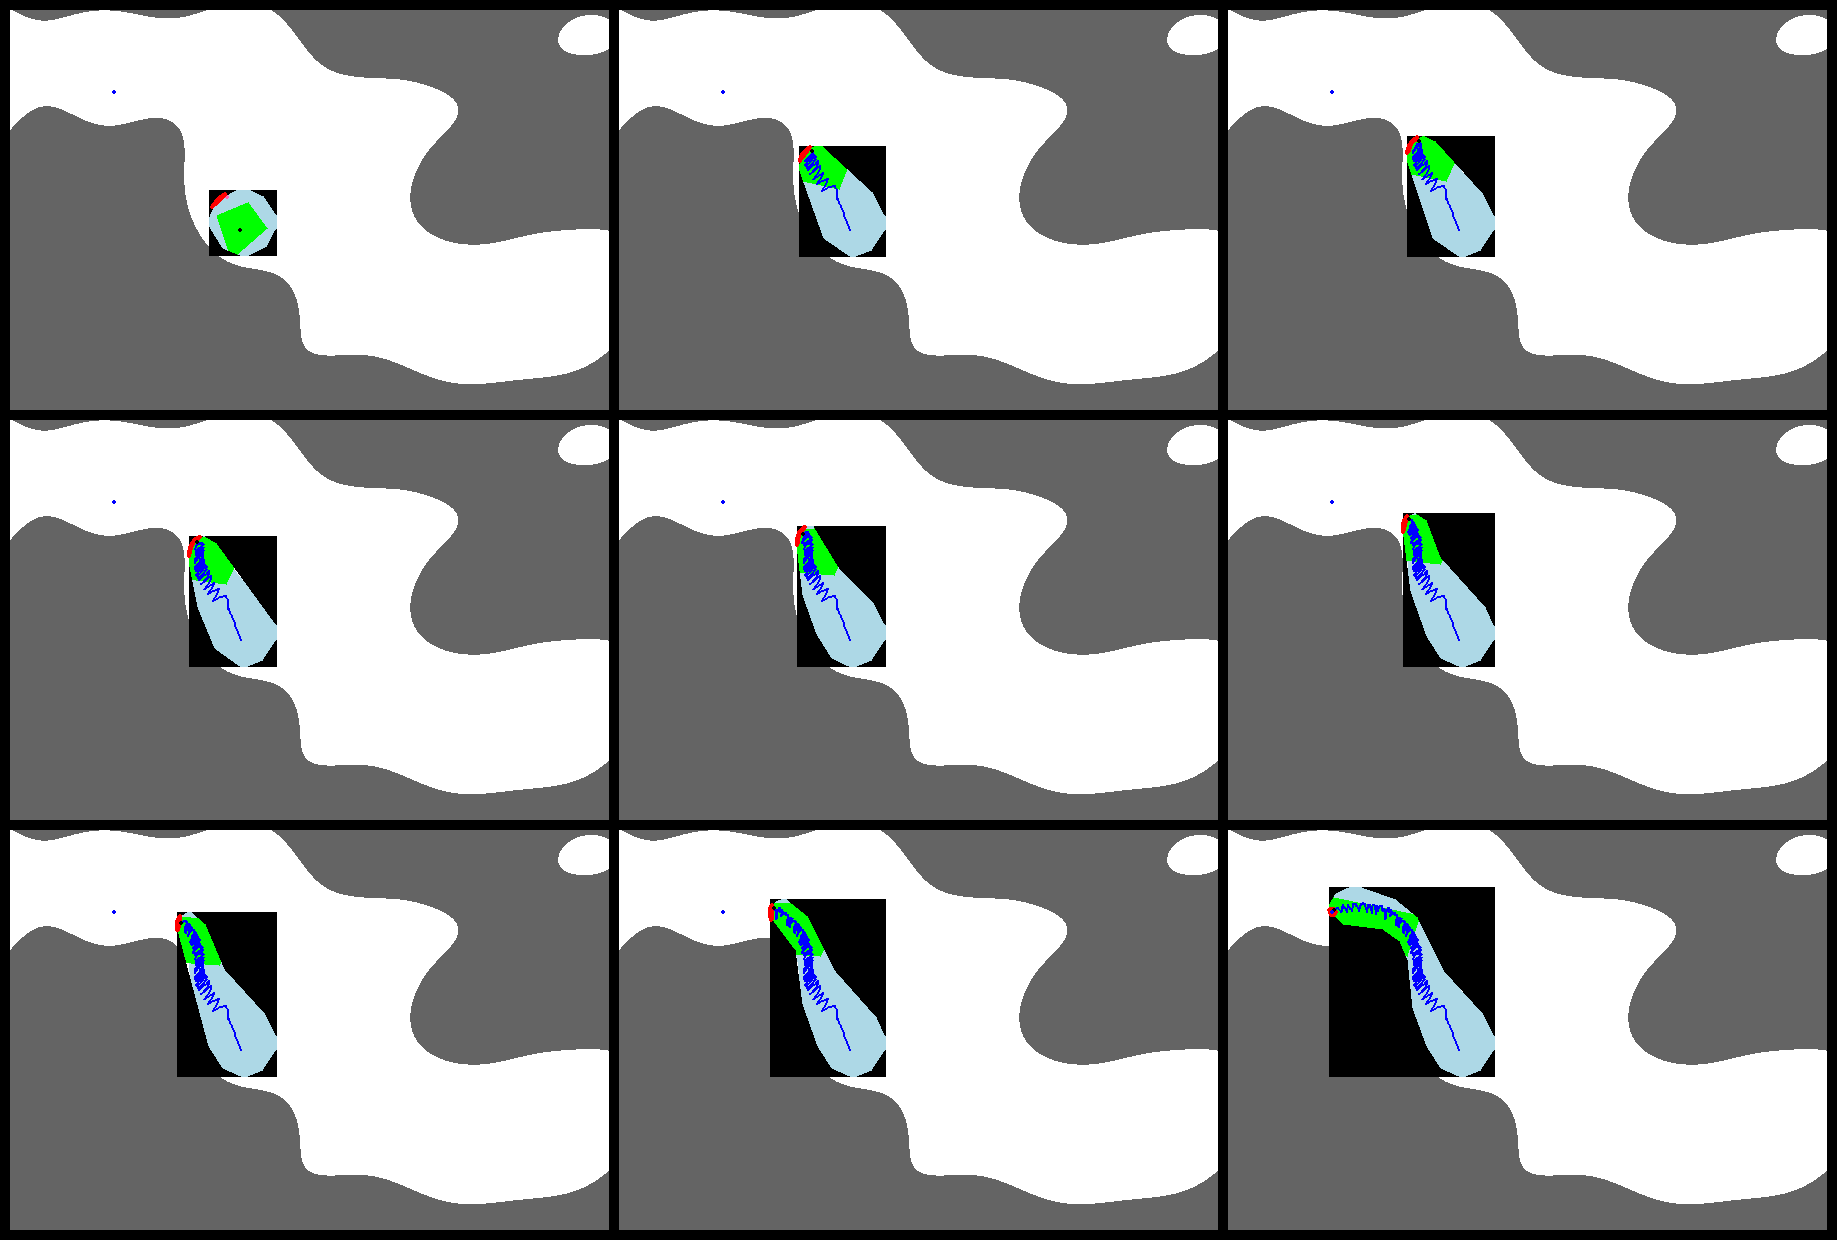
\includegraphics[width=1\linewidth]{figures/navigation.png}
    \caption{Nine frames showing the progression of the navigation task around a risk zone at evenly spaced intervals. Gray zones represent areas where traversability f(x) is less than 1000.}
    \label{fig:navigation}
\end{figure}

\begin{figure}[h]
    \centering
    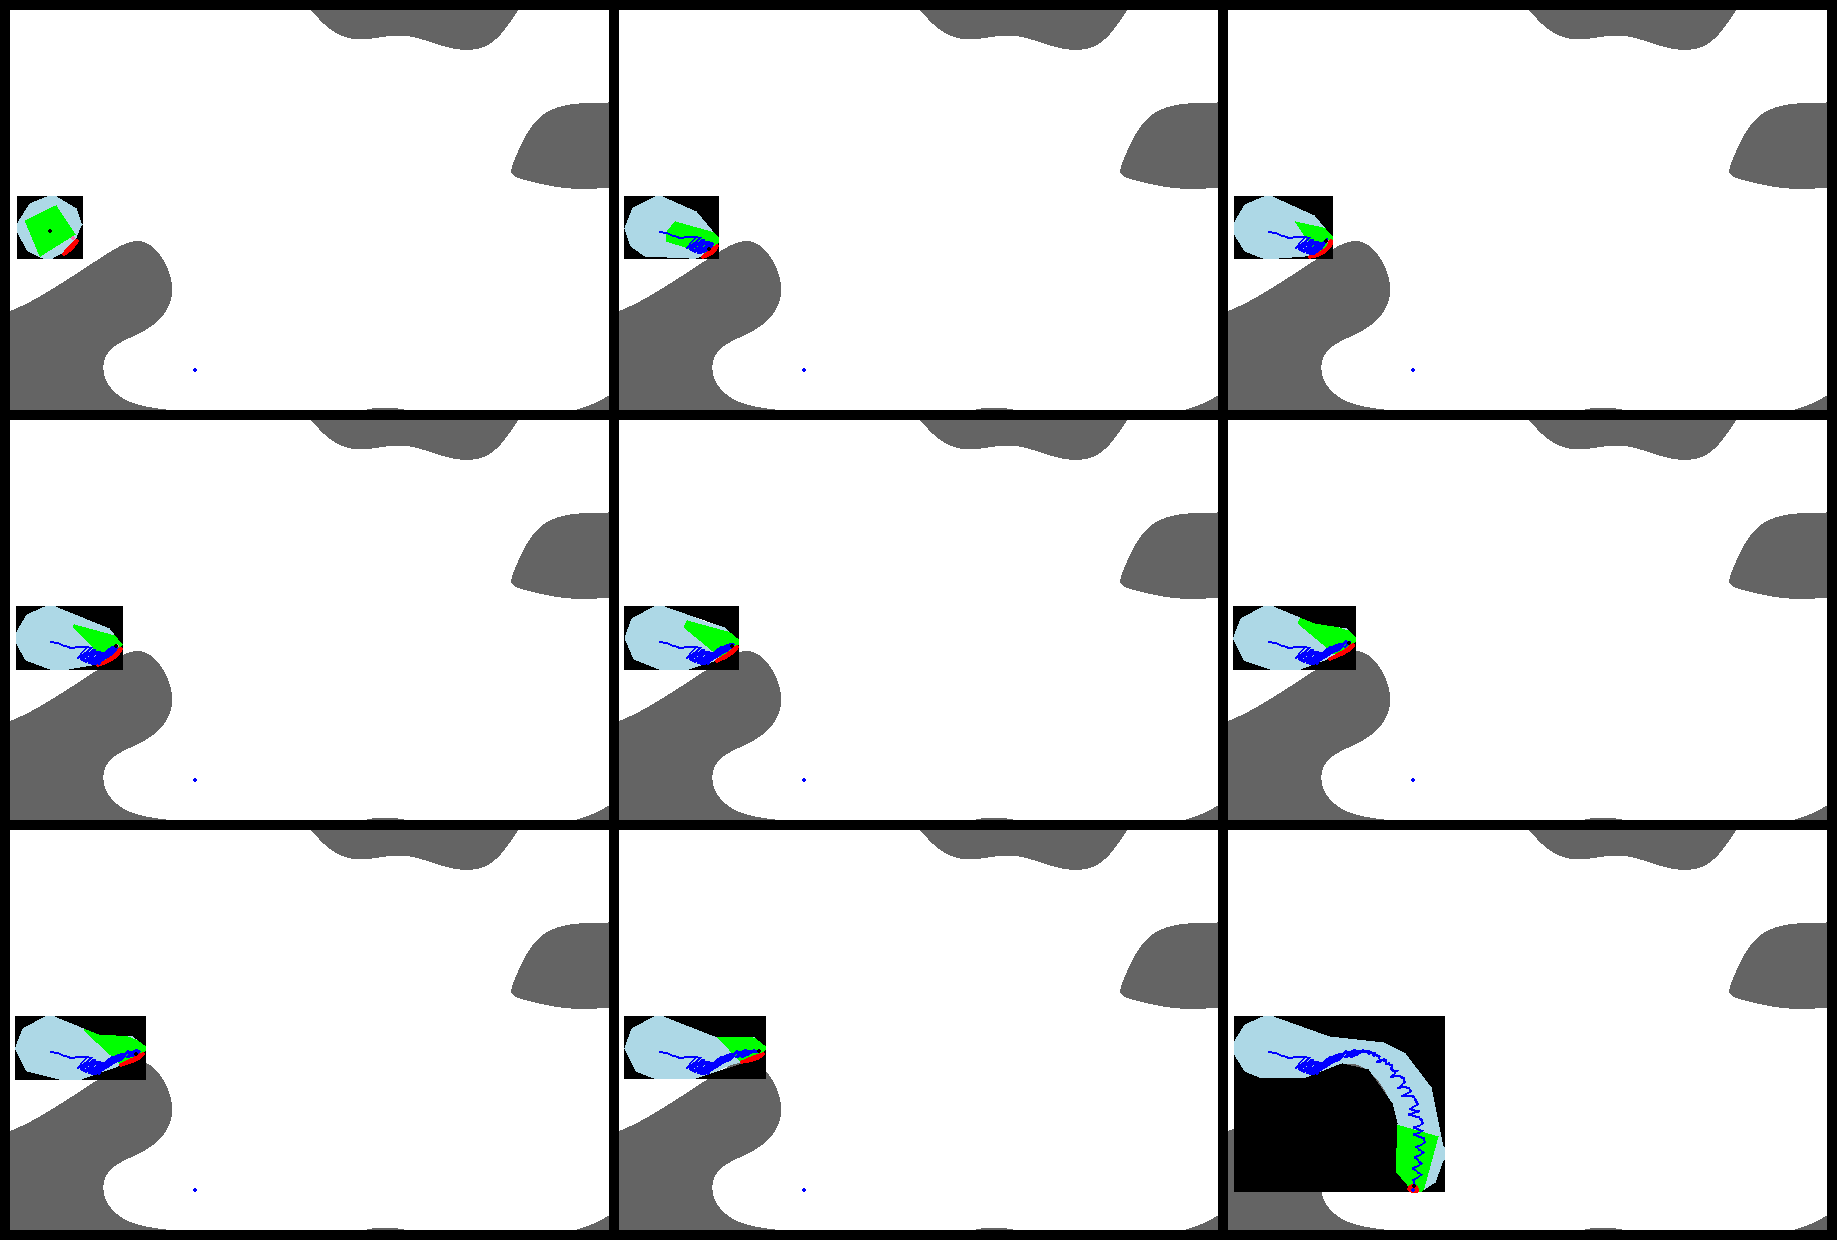
\includegraphics[width=1\linewidth]{figures/navigation2.png}
    \caption{Nine frames showing the progression of the navigation task around a risk zone at evenly spaced intervals. Gray zones represent areas where traversability f(x) is less than 500.}
    \label{fig:navigation2}
\end{figure}

The complete navigation path was generated after 210 and 461 planning iterations, where each iteration includes one terrain measurement and safe set update. Initially, the robot rapidly expands the explored safe zone until encountering regions approaching the risk threshold. As the robot gets closer to the risk zone, the algorithm selects exploration points around the periphery of the high-risk area, ensuring the robot maintains a safe distance from dangerous terrain while progressing toward the goal. Then, when the robot passes the risk area, each safe set expansion becomes much larger and less constrained, reaching the goal quickly. 

A learned safe path can be reused in a subsequent navigation task, as can be seen in the following test scenario.

\subsubsection{Traversing Across Known Safe Area to Reach Opposite Side}
\begin{figure}[h]
    \centering
    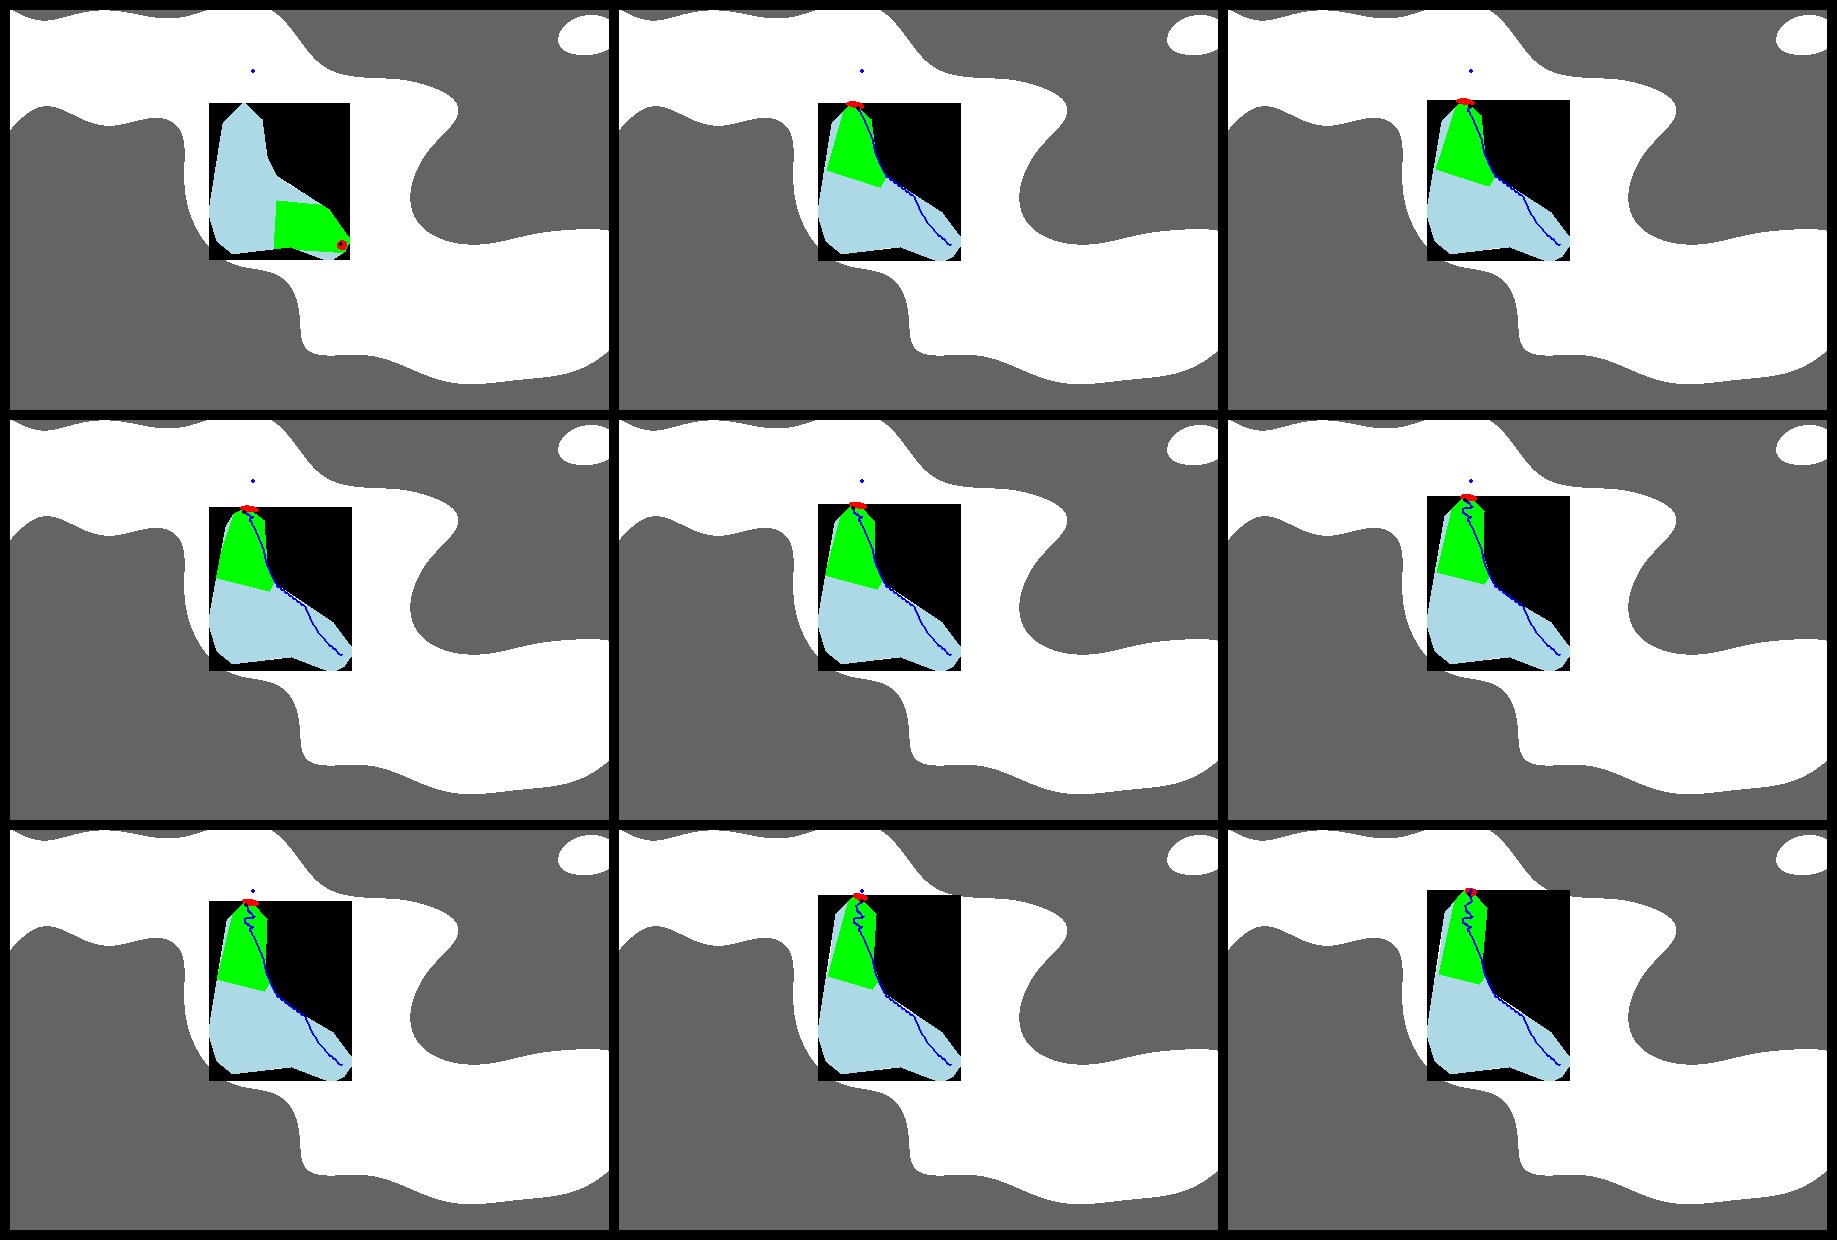
\includegraphics[width=1\linewidth]{figures/known.png}
    \caption{Nine frames showing the progression of the navigation task at evenly spaced intervals. Gray zones represent areas where traversability f(x) is less than 1000.}
    \label{fig:known}
\end{figure}

This experiment demonstrates how the robot leverages previously acquired knowledge about safe regions. After exploring for some time and creating a larger known safe area, the robot was positioned at a new starting point with the goal of reaching the opposite side of the environment.

As illustrated in \autoref{fig:known}, the robot efficiently navigates across a previously learned safe corridor around the high-risk area. This traversal completed in only 10 iterations, as the robot was able to utilize the large safe zone to travel without stopping, only beginning to take new measurements after reaching the first sub-goal. 

The robot maintains its safety-conscious behavior throughout the traversal, staying within the previously established safe zones and avoiding unnecessary re-exploration of the environment. This capability is particularly valuable in applications where repeated navigation through partially known environments is required, such as periodic inspection tasks or multi-objective missions.

\subsubsection{Exploring Without a Goal in Mind}

\begin{figure}[h]
    \centering
    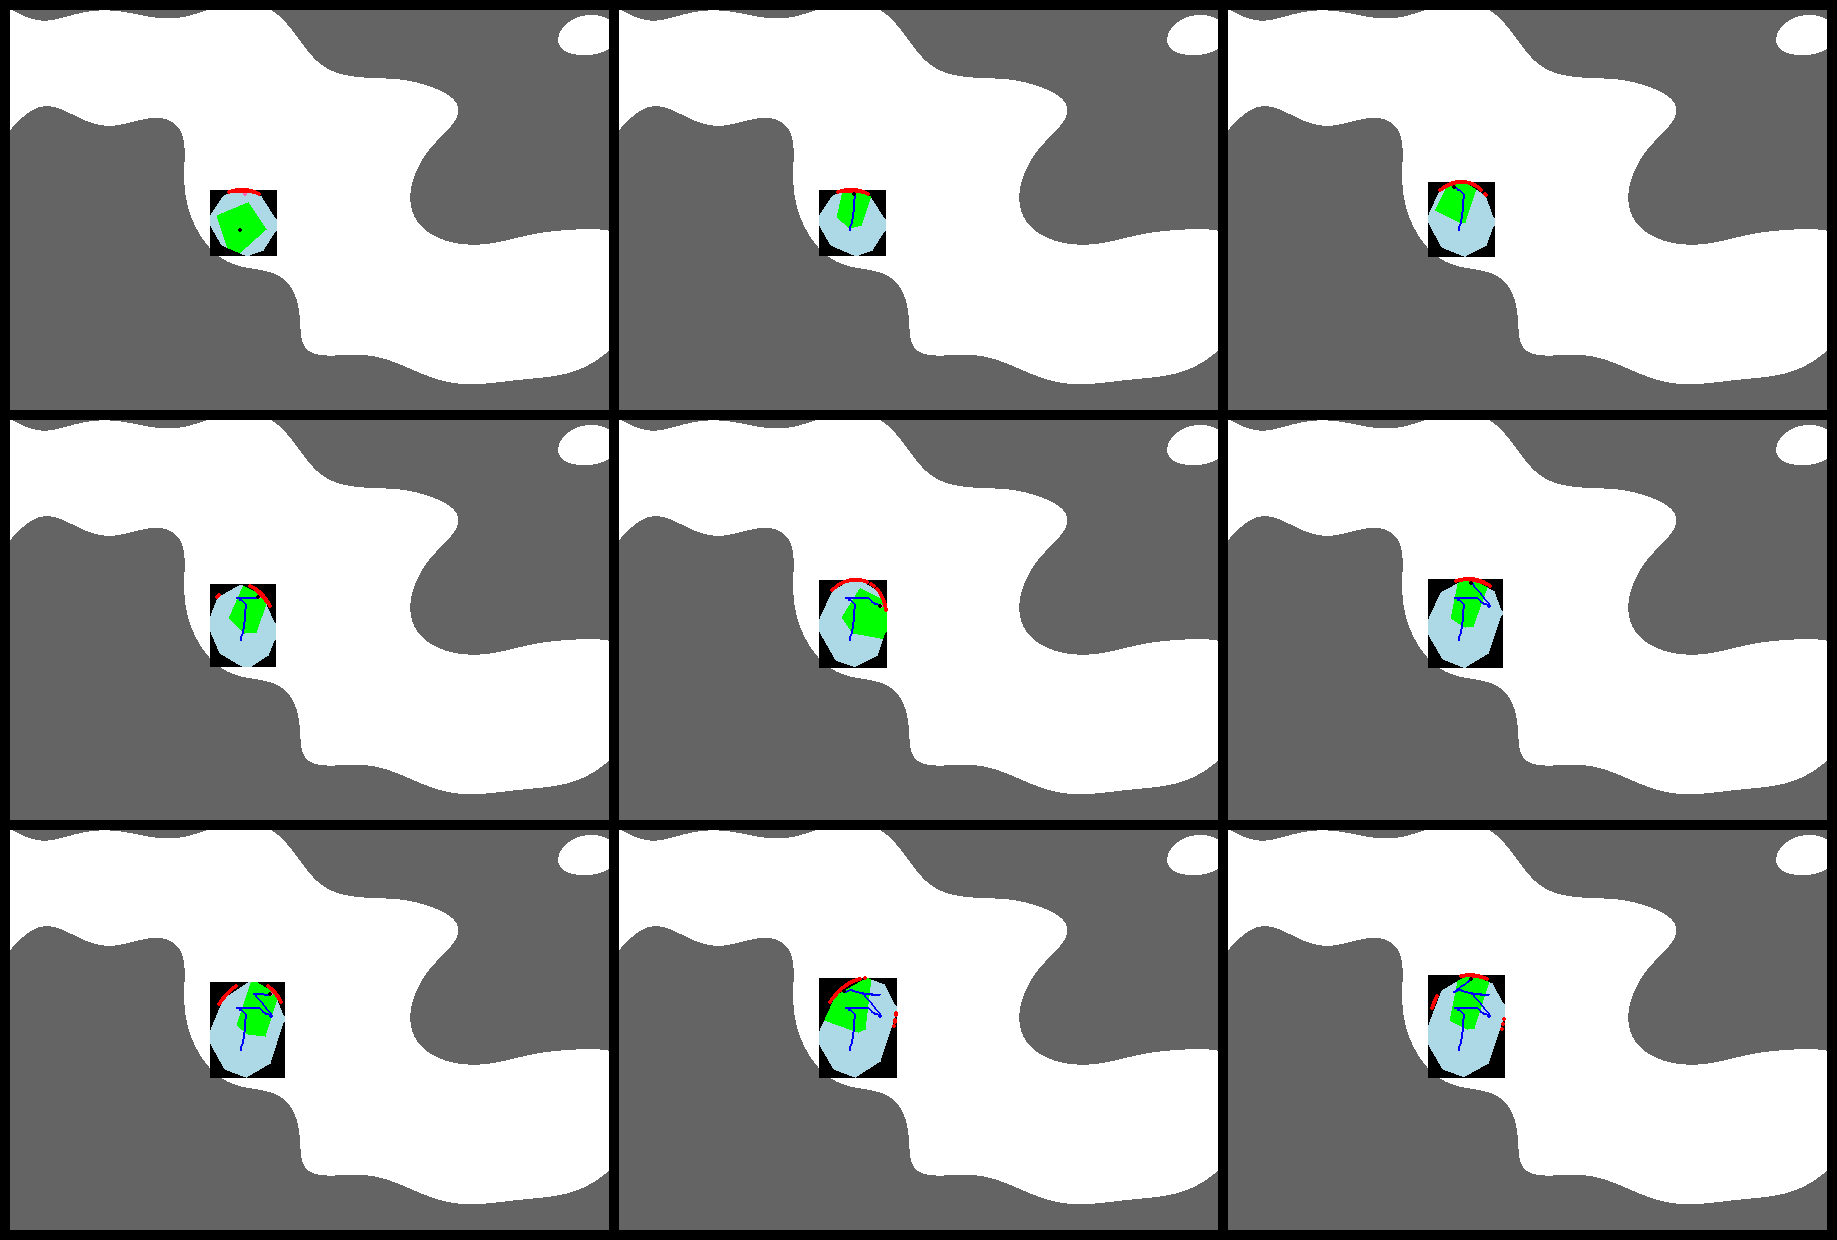
\includegraphics[width=1\linewidth]{figures/explore.png}
    \caption{The first nine frames of the exploration task. Gray zones represent areas where traversability f(x) is less than 1000.}
    \label{fig:explore}
\end{figure}

\begin{figure}[h]
    \centering
    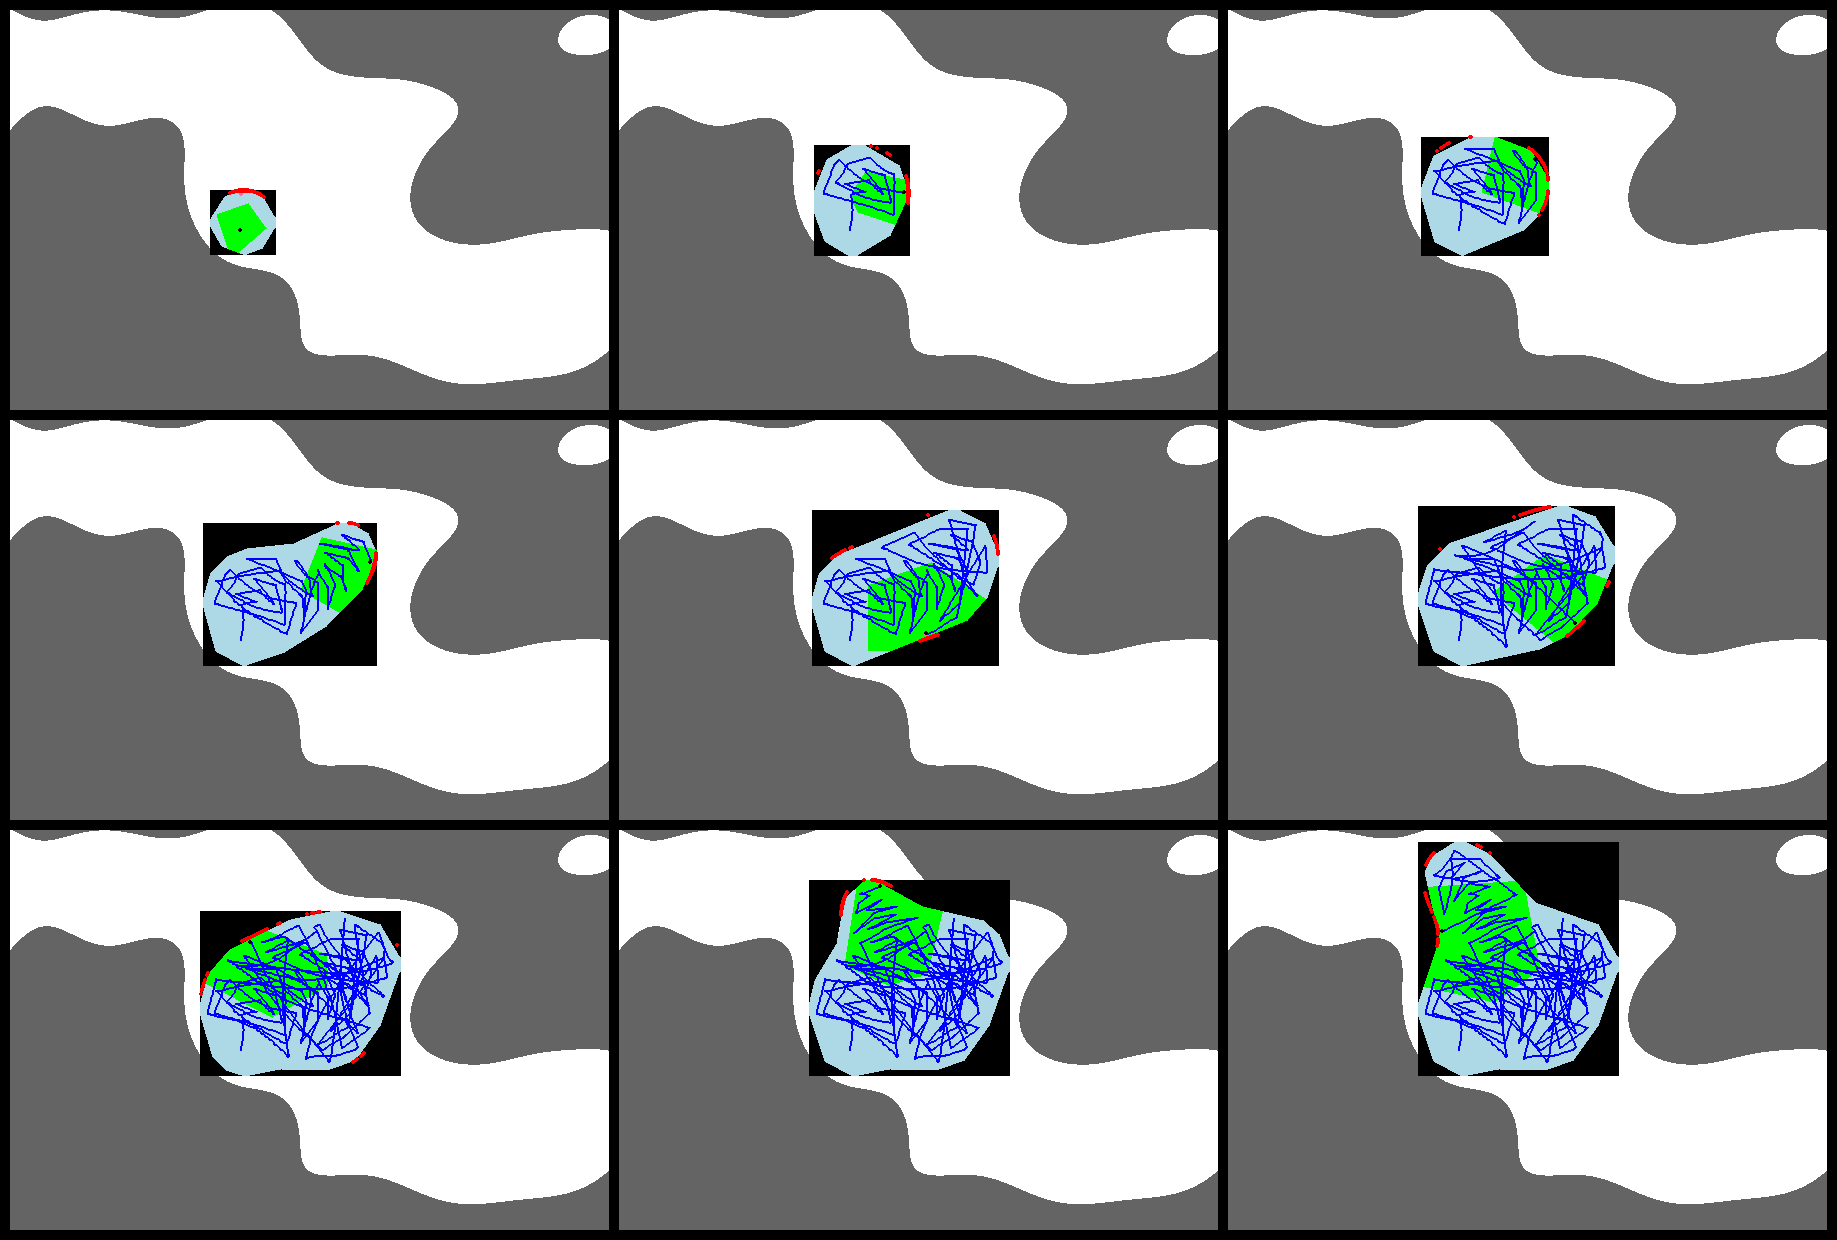
\includegraphics[width=1\linewidth]{figures/explorefull.png}
    \caption{Nine frames showing the overall progression of the exploration task. Gray zones represent areas where traversability f(x) is less than 1000.}
    \label{fig:explorefull}
\end{figure}

When given the task to simply explore without a goal in mind, the robot selects sub-goals that maximize terrain uncertainty reduction, independent of any goal location. As can be seen in \autoref{fig:explore}, the robot selects points where the most information can be revealed about the map. It expands the safe zone as quickly as possible, resulting in a larger known area, shown in \autoref{fig:explorefull}, faster than in a goal-oriented navigation task. 

This exploration behavior demonstrates how \algoname\ can be applied to general environmental mapping tasks without requiring predefined destinations. The algorithm prioritizes points at the frontiers of the known safe region, systematically expanding the mapped area while maintaining safety constraints. In just 9 iterations, the robot has successfully mapped a significant portion of the accessible environment, creating a comprehensive safety map.

This scenario proves particularly useful for robots that have just deployed in a small safe area without prior inspection of the surroundings. Running an exploration task before assigning an explicit navigation goal allows the system to build a safety model of the environment, which can subsequently enhance the efficiency of goal-directed tasks by reducing the need for cautious exploration during navigation.

\subsection{Comparisons to Baseline Methods}

\subsubsection{Comparison to Reactive Baseline Navigation}

To further contextualize the performance of \algoname, we compare it to a standard reactive navigation baseline shown in \autoref{fig:baseline} that lacks probabilistic terrain modeling and safe set reasoning. The baseline method operates under the assumption that the robot can safely navigate directly toward the goal along the shortest Euclidean path, adjusting only when immediate obstacles are encountered.

This naive strategy fails to account for terrain risk unless the risk manifests as an explicit obstacle in a local sensing field. As a result, when the shortest path intersects a high-risk region not detectable by general sensing methods, the robot proceeds directly through it, leading to unsafe behavior and frequent failures. In contrast, \algoname\ actively models the risk of terrain using a Gaussian Process and expands a certified safe set around the robot. It selects subgoals based not solely on distance but on estimated safety and uncertainty.

The introduction of the safe zone representation and confidence-based subgoal selection allows \algoname\ to anticipate and avoid unsafe terrain even before it is physically encountered. Across all scenarios presented in this chapter—including those with complex terrain topographies and non-convex risk zones—\algoname\ achieved a 0\% failure rate, provided that the hyperparameters (e.g., Lipschitz coefficient $L$, exploration parameter $\beta$) were appropriately tuned to accurately reflect the underlying terrain characteristics.

\begin{figure}
    \centering
    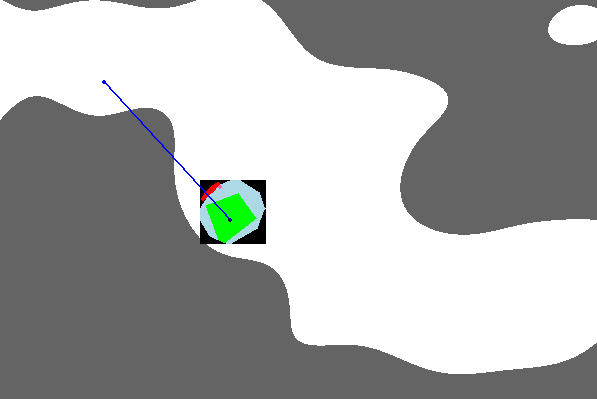
\includegraphics[width=0.7\linewidth]{figures/baseline.png}
    \caption{The baseline navigation result, as shown for the scenario in \autoref{fig:navigation}.}
    \label{fig:baseline}
\end{figure}

This performance contrast highlights the fundamental advantage of combining proprioceptive sensing, probabilistic terrain modeling, and confidence-aware planning. Without these components, as shown in the baseline strategy, the robot is prone to entering unsafe terrain. With \algoname, the robot instead exhibits foresight, adaptability, and safety-conscious behavior—capabilities essential for autonomous planetary exploration in uncertain and deformable environments.

\begin{table}[h]
\centering
\caption{Performance Comparison Between \algoname\ and Reactive Baseline}
\label{tab:performance_comparison}
\begin{tabular}{|p{5cm}|p{5cm}|p{5cm}|}
\hline
\textbf{Metric} & \textbf{Reactive Baseline} & \textbf{\algoname} \\
\hline
Success Rate & Low; guaranteed failure when passing risky terrain & High; 0\% failure rate with accurately tuned hyperparameters \\
\hline
Path Length & Shortest-path by default, but often unsafe or infeasible & Slightly longer paths that avoid risk zones; consistently feasible \\
\hline
Computational Efficiency & Low; minimal computation, but unsafe & Moderate; additional overhead for GP and confidence checks, but manageable in real time \\
\hline
\end{tabular}
\end{table}

\subsubsection{Comparison to Prior Gaussian Process-Based Planning}
\label{sec:comparison_prior}

While the reactive baseline illustrates the importance of terrain modeling and safety-aware planning, it is also valuable to compare \algoname\ against more structured, probabilistically informed methods. One such method is the framework proposed by \textcite{leininger2024gaussianprocessbasedtraversabilityanalysis}, which combines Sparse Gaussian Processes (SGP) with RRT*-based motion planning. This approach offers global terrain reasoning and path planning capabilities using uncertainty-aware models. However, \algoname\ distinguishes itself through a number of architectural and operational design choices that make it more suitable for granular terrain exploration using local feedback.

\paragraph{Planning Strategy.} \textcite{leininger2024gaussianprocessbasedtraversabilityanalysis}'s approach constructs global paths to the goal using RRT* over a probabilistic terrain cost map. This requires maintaining and updating a global terrain estimate and is most effective in structured or semi-known environments. In contrast, \algoname\ takes a reactive planning approach that forgoes global path computation in favor of incremental, confidence-aware subgoal selection from a locally expanding safe set. This supports greater flexibility in dynamically evolving or unknown environments.

\paragraph{Uncertainty Handling.} While both methods utilize Gaussian Process models to estimate terrain risk and uncertainty, \algoname\ directly incorporates the GP confidence bounds into its decision-making loop. The confidence intervals define both the safe and expander sets that determine feasible and informative next steps. In the SGP-RRT* formulation, uncertainty is treated as a scalar cost modulation rather than as a constraint mechanism to enforce safety under uncertainty.

\paragraph{Sensing Assumptions.} A critical difference lies in sensing modality. The SGP-RRT* planner assumes access to exteroceptive observations, such as visual or remote terrain features, to update the GP model. In contrast, \algoname\ is built for scenarios in which such sensing may be unavailable or unreliable. It relies solely on proprioceptive feedback gathered through direct terrain interaction—making it particularly well-suited for planetary missions in dust-obscured or visually degraded environments.

Taken together, these distinctions highlight how \algoname\ extends the capabilities of uncertainty-aware terrain modeling into domains where traditional planning pipelines fall short. The integration of proprioceptive sensing, real-time safe set expansion, and local control makes \algoname\ more resilient in scenarios where structural assumptions break down.


\section{Conclusions from Simulation Trials}

The simulation experiments presented in this chapter validate the intended capabilities of \algoname\ under a variety of terrain conditions and risk scenarios. The robot successfully performs uncertainty-aware navigation around hazardous terrain, reuses previously acquired safe knowledge to complete tasks more efficiently, and performs autonomous environmental mapping using only local proprioceptive measurements.